\documentclass[a4paper,justified,final,twoside,nobib]{tufte-book}

\hypersetup{colorlinks}% uncomment this line if you prefer colored hyperlinks (e.g., for onscreen viewing)

%%
% Book metadata
\title{A\\Machine Learning\\Handbook\thanks{Thanks to Edward R.~Tufte for his inspiration.}}
\author[]{}
\publisher{Publisher of This Book}

%%
% Automated bibliography management
\usepackage{natbib}
\setcitestyle{authoryear}

%%
% If they're installed, use Bergamo and Chantilly from www.fontsite.com.
% They're clones of Bembo and Gill Sans, respectively.
%\IfFileExists{bergamo.sty}{\usepackage[osf]{bergamo}}{}% Bembo
%\IfFileExists{chantill.sty}{\usepackage{chantill}}{}% Gill Sans

\usepackage{microtype}

%%
% Just some sample text
\usepackage{lipsum}
\usepackage{soul}
%%
% For nicely typeset tabular material
\usepackage{booktabs}
\usepackage{pdfpages}

%%
% For graphics / images
\usepackage{graphicx}
\setkeys{Gin}{width=\linewidth,totalheight=\textheight,keepaspectratio}
\graphicspath{{graphics/}}

% The fancyvrb package lets us customize the formatting of verbatim
% environments.  We use a slightly smaller font.
\usepackage{fancyvrb}
\fvset{fontsize=\normalsize}

%%
% Prints argument within hanging parentheses (i.e., parentheses that take
% up no horizontal space).  Useful in tabular environments.
\newcommand{\hangp}[1]{\makebox[0pt][r]{(}#1\makebox[0pt][l]{)}}

%%
% Prints an asterisk that takes up no horizontal space.
% Useful in tabular environments.
\newcommand{\hangstar}{\makebox[0pt][l]{*}}

%%
% Prints a trailing space in a smart way.
\usepackage{xspace}

%%
% Some shortcuts for Tufte's book titles.  The lowercase commands will
% produce the initials of the book title in italics.  The all-caps commands
% will print out the full title of the book in italics.
\newcommand{\vdqi}{\textit{VDQI}\xspace}
\newcommand{\ei}{\textit{EI}\xspace}
\newcommand{\ve}{\textit{VE}\xspace}
\newcommand{\be}{\textit{BE}\xspace}
\newcommand{\VDQI}{\textit{The Visual Display of Quantitative Information}\xspace}
\newcommand{\EI}{\textit{Envisioning Information}\xspace}
\newcommand{\VE}{\textit{Visual Explanations}\xspace}
\newcommand{\BE}{\textit{Beautiful Evidence}\xspace}
\newcommand{\ics}{\smallcaps{ICS5110 Applied Machine Learning\xspace}}

\newcommand{\TL}{Tufte-\LaTeX\xspace}

% Prints the month name (e.g., January) and the year (e.g., 2008)
\newcommand{\monthyear}{%
  \ifcase\month\or January\or February\or March\or April\or May\or June\or
  July\or August\or September\or October\or November\or
  December\fi\space\number\year
}

% Prints an epigraph and speaker in sans serif, all-caps type.
\newcommand{\openepigraph}[2]{%
  %\sffamily\fontsize{14}{16}\selectfont
  \begin{fullwidth}
  \sffamily\large
  \begin{doublespace}
  \noindent\allcaps{#1}\\% epigraph
  \noindent\allcaps{#2}% author
  \end{doublespace}
  \end{fullwidth}
}

% Inserts a blank page
\newcommand{\blankpage}{\newpage\hbox{}\thispagestyle{empty}\newpage}

\usepackage{units}

% Typesets the font size, leading, and measure in the form of 10/12x26 pc.
\newcommand{\measure}[3]{#1/#2$\times$\unit[#3]{pc}}

% Macros for typesetting the documentation
\newcommand{\hlred}[1]{\textcolor{Maroon}{#1}}% prints in red
\newcommand{\hangleft}[1]{\makebox[0pt][r]{#1}}
\newcommand{\hairsp}{\hspace{1pt}}% hair space
\newcommand{\hquad}{\hskip0.5em\relax}% half quad space
\newcommand{\TODO}{\textcolor{red}{\bf TODO!}\xspace}
\newcommand{\ie}{\textit{i.\hairsp{}e.}\xspace}
\newcommand{\eg}{\textit{e.\hairsp{}g.}\xspace}
\newcommand{\na}{\quad--}% used in tables for N/A cells
\providecommand{\XeLaTeX}{X\lower.5ex\hbox{\kern-0.15em\reflectbox{E}}\kern-0.1em\LaTeX}
\newcommand{\tXeLaTeX}{\XeLaTeX\index{XeLaTeX@\protect\XeLaTeX}}
% \index{\texttt{\textbackslash xyz}@\hangleft{\texttt{\textbackslash}}\texttt{xyz}}
\newcommand{\tuftebs}{\symbol{'134}}% a backslash in tt type in OT1/T1
\newcommand{\doccmdnoindex}[2][]{\texttt{\tuftebs#2}}% command name -- adds backslash automatically (and doesn't add cmd to the index)
\newcommand{\doccmddef}[2][]{%
  \hlred{\texttt{\tuftebs#2}}\label{cmd:#2}%
  \ifthenelse{\isempty{#1}}%
    {% add the command to the index
      \index{#2 command@\protect\hangleft{\texttt{\tuftebs}}\texttt{#2}}% command name
    }%
    {% add the command and package to the index
      \index{#2 command@\protect\hangleft{\texttt{\tuftebs}}\texttt{#2} (\texttt{#1} package)}% command name
      \index{#1 package@\texttt{#1} package}\index{packages!#1@\texttt{#1}}% package name
    }%
}% command name -- adds backslash automatically
\newcommand{\doccmd}[2][]{%
  \texttt{\tuftebs#2}%
  \ifthenelse{\isempty{#1}}%
    {% add the command to the index
      \index{#2 command@\protect\hangleft{\texttt{\tuftebs}}\texttt{#2}}% command name
    }%
    {% add the command and package to the index
      \index{#2 command@\protect\hangleft{\texttt{\tuftebs}}\texttt{#2} (\texttt{#1} package)}% command name
      \index{#1 package@\texttt{#1} package}\index{packages!#1@\texttt{#1}}% package name
    }%
}% command name -- adds backslash automatically
\newcommand{\docopt}[1]{\ensuremath{\langle}\textrm{\textit{#1}}\ensuremath{\rangle}}% optional command argument
\newcommand{\docarg}[1]{\textrm{\textit{#1}}}% (required) command argument
\newenvironment{docspec}{\begin{quotation}\ttfamily\parskip0pt\parindent0pt\ignorespaces}{\end{quotation}}% command specification environment
\newcommand{\docenv}[1]{\texttt{#1}\index{#1 environment@\texttt{#1} environment}\index{environments!#1@\texttt{#1}}}% environment name
\newcommand{\docenvdef}[1]{\hlred{\texttt{#1}}\label{env:#1}\index{#1 environment@\texttt{#1} environment}\index{environments!#1@\texttt{#1}}}% environment name
\newcommand{\docpkg}[1]{\texttt{#1}\index{#1 package@\texttt{#1} package}\index{packages!#1@\texttt{#1}}}% package name
\newcommand{\doccls}[1]{\texttt{#1}}% document class name
\newcommand{\docclsopt}[1]{\texttt{#1}\index{#1 class option@\texttt{#1} class option}\index{class options!#1@\texttt{#1}}}% document class option name
\newcommand{\docclsoptdef}[1]{\hlred{\texttt{#1}}\label{clsopt:#1}\index{#1 class option@\texttt{#1} class option}\index{class options!#1@\texttt{#1}}}% document class option name defined
\newcommand{\docmsg}[2]{\bigskip\begin{fullwidth}\noindent\ttfamily#1\end{fullwidth}\medskip\par\noindent#2}
\newcommand{\docfilehook}[2]{\texttt{#1}\index{file hooks!#2}\index{#1@\texttt{#1}}}
\newcommand{\doccounter}[1]{\texttt{#1}\index{#1 counter@\texttt{#1} counter}}

% Generates the index
\usepackage{makeidx}
\makeindex

\usepackage{tikz}

\begin{document}
	\begingroup
	\thispagestyle{empty}
	\begin{tikzpicture}[remember picture,overlay]
	\node[inner sep=0pt] (background) at (current page.center) {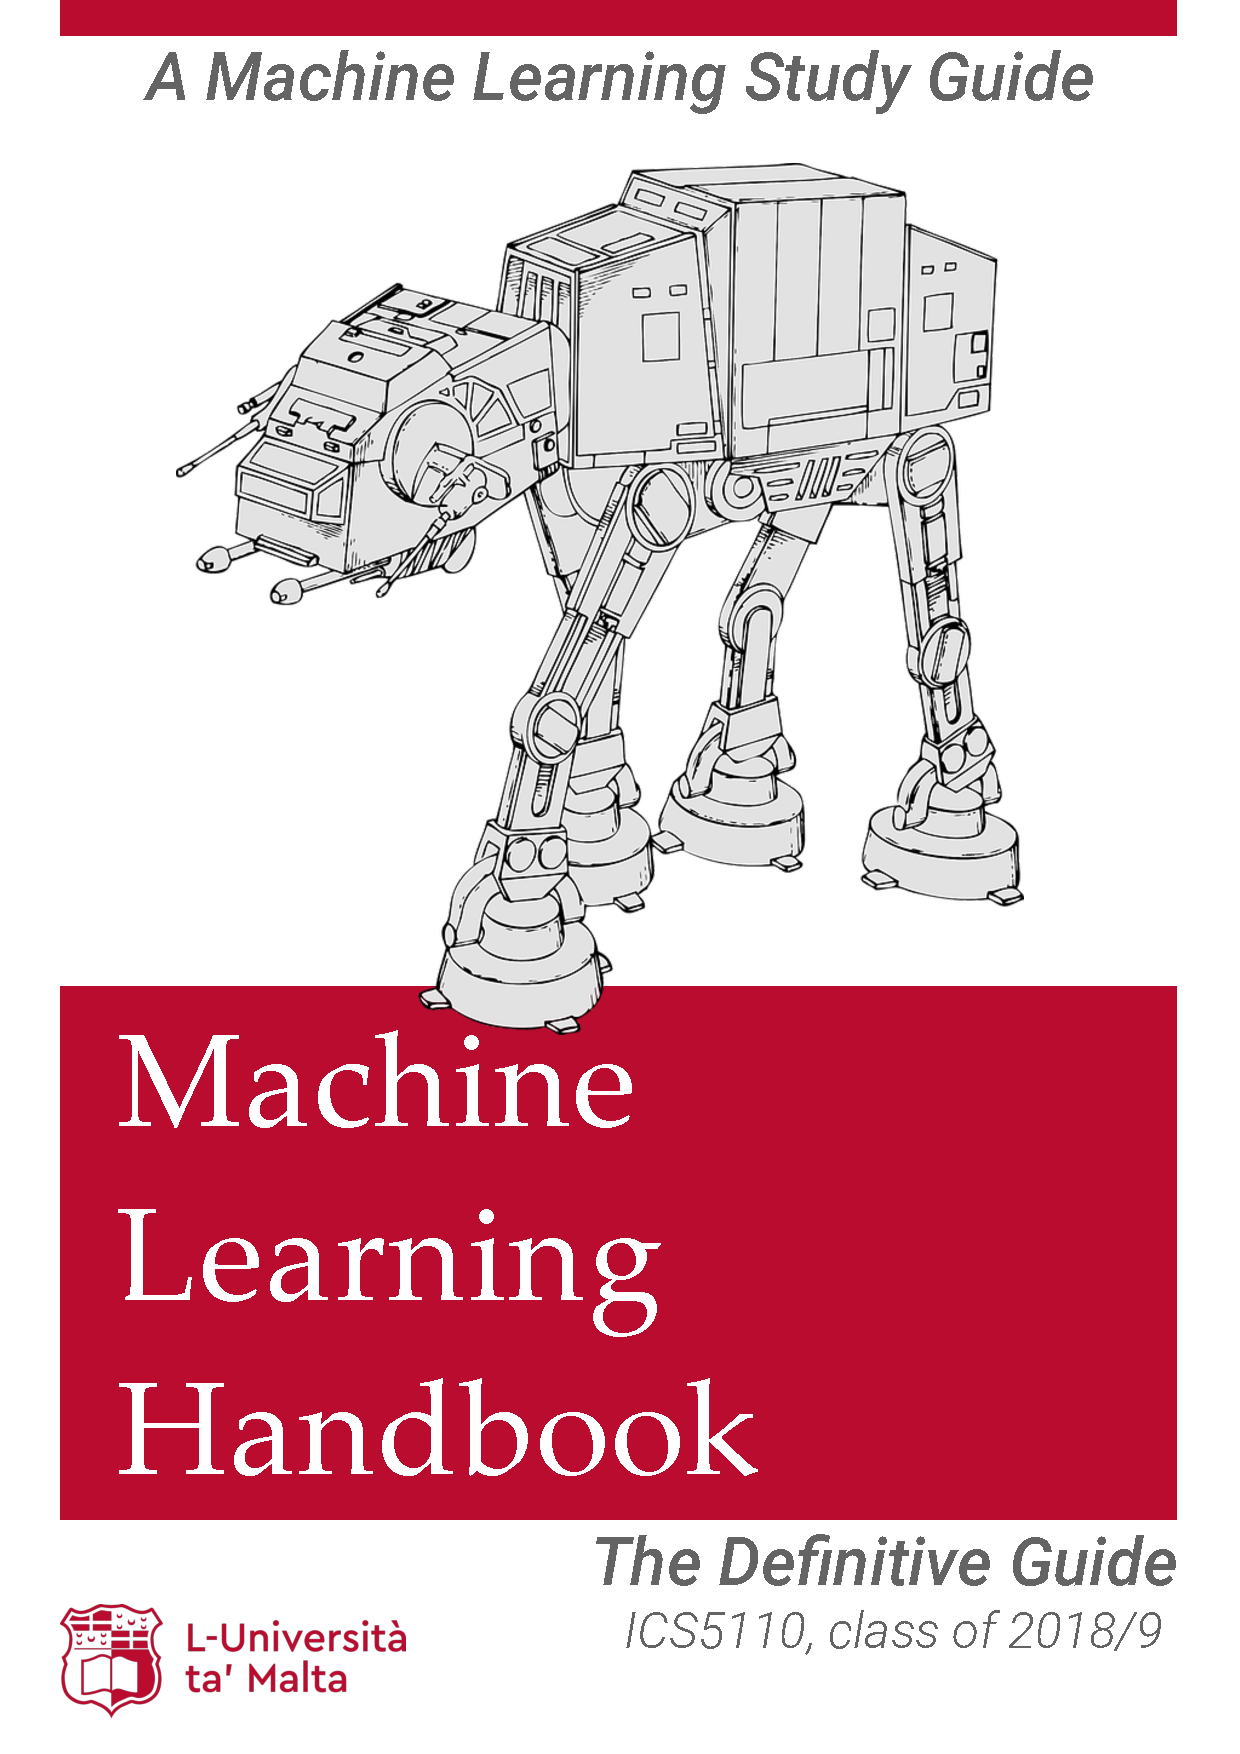
\includegraphics[width=\paperwidth]{cover/cover_oreilly_style.pdf}};
	%%\draw (current page.center) node [fill=ocre!30!white,fill opacity=0.6,text opacity=1,inner sep=1cm]{\Huge\centering\bfseries\sffamily\parbox[c][][t]{\paperwidth}{\centering The Search for a Title\\[15pt] % Book title
	%%{\Large A Profound Subtitle}\\[20pt] % Subtitle
	%%{\huge Dr. John Smith}}}; % Author name
	\end{tikzpicture}
	\vfill
	\endgroup
	

% Front matter
\frontmatter

% r.3 full title page
%% \maketitle


% v.4 copyright page
\newpage
\begin{fullwidth}
~\vfill
\thispagestyle{empty}
\setlength{\parindent}{0pt}
\setlength{\parskip}{\baselineskip}
\begin{figure*}[h]
	
\includegraphics[width=2.5in]{UMLOGO_redRGB.png}%
\end{figure*}

\par Copyright \copyright\ \the\year\ \ics\ class of 2018/9, University of Malta.

\par\smallcaps{Jean-Paul Ebejer, Dylan Seychell, Lara Marie Demajo, Patrick Bezzina \hl{ADD YOUR NAME TO THIS LIST} } %TODO

\par Licensed under the Apache License, Version 2.0 (the ``License''); you may not
use this file except in compliance with the License. You may obtain a copy
of the License at \url{http://www.apache.org/licenses/LICENSE-2.0}. Unless
required by applicable law or agreed to in writing, software distributed
under the License is distributed on an \smallcaps{``AS IS'' BASIS, WITHOUT
WARRANTIES OR CONDITIONS OF ANY KIND}, either express or implied. See the
License for the specific language governing permissions and limitations
under the License.\index{license}

\par\textit{First printing, \monthyear}
\end{fullwidth}

% r.5 contents
\tableofcontents

%%\listoffigures

%%\listoftables

% r.9 introduction
\cleardoublepage
\chapter{Introduction}

This book explains popular Machine Learning terms.  We focus to explain each term comprehensively, through the use of examples and diagrams.  The description of each term is written by a student sitting in for \ics\footnote{\url{https://www.um.edu.mt/courses/studyunit/ICS5110}} at the University of Malta (class 2018/2019).  This study-unit is part of the MSc.\ in AI offered by the Department of Artificial Intelligence, Faculty of ICT.

%%
% Start the main matter (normal chapters)
\mainmatter

%% JP's example file -- file must be stored in directory "terms" and have
%% the term and initials of the student in the filename.
%% \chapter[On the Use of the tufte-book Document Class]{On the Use of the \texttt{tufte-book} Document Class}
\label{ch:tufte-book}



The \TL document classes define a style similar to the
style Edward Tufte uses in his books and handouts.  Tufte's style is known
for its extensive use of sidenotes, tight integration of graphics with
text, and well-set typography.  This document aims to be at once a
demonstration of the features of the \TL document classes
and a style guide to their use.

\section{Page Layout}\label{sec:page-layout}
\subsection{Headings}\label{sec:headings}\index{headings}
This style provides \textsc{a}- and \textsc{b}-heads (that is,
\Verb|\section| and \Verb|\subsection|), demonstrated above.

If you need more than two levels of section headings, you'll have to define
them yourself at the moment; there are no pre-defined styles for anything below
a \Verb|\subsection|.  As Bringhurst points out in \textit{The Elements of
Typographic Style},\cite{Bringhurst2005} you should ``use as many levels of
headings as you need: no more, and no fewer.''

The \TL classes will emit an error if you try to use
\linebreak\Verb|\subsubsection| and smaller headings.

% let's start a new thought -- a new section
\newthought{In his later books},\cite{Tufte2006} Tufte
starts each section with a bit of vertical space, a non-indented paragraph,
and sets the first few words of the sentence in \textsc{small caps}.  To
accomplish this using this style, use the \doccmddef{newthought} command:
\begin{docspec}
  \doccmd{newthought}\{In his later books\}, Tufte starts\ldots
\end{docspec}

\bigskip
\begin{center}
\footnotesize
\begin{tabular}{lllll}
\toprule
Feature & \vdqi & \ei & \ve & \be \\
\midrule
Author & & & & \\
\quad Typeface & serif   & serif   & serif   & sans serif \\
\quad Style    & italics & italics & italics & upright, caps \\
\quad Size     & 24 pt   & 20 pt   & 20 pt   & 20 pt \\
\addlinespace
Title & & & & \\
\quad Typeface & serif   & serif   & serif   & sans serif \\
\quad Style    & upright & italics & upright & upright, caps \\
\quad Size     & 36 pt   & 48 pt   & 48 pt   & 36 pt \\
\addlinespace
Subtitle & & & & \\
\quad Typeface & \na     & \na     & serif   & \na \\
\quad Style    & \na     & \na     & upright & \na \\
\quad Size     & \na     & \na     & 20 pt   & \na \\
\addlinespace
Edition & & & & \\
\quad Typeface & sans serif    & \na  & \na  & \na \\
\quad Style    & upright, caps & \na  & \na  & \na \\
\quad Size     & 14 pt         & \na  & \na  & \na \\
\addlinespace
Publisher & & & & \\
\quad Typeface & serif   & serif   & serif   & sans serif \\
\quad Style    & italics & italics & italics & upright, caps \\
\quad Size     & 14 pt   & 14 pt   & 14 pt   & 14 pt \\
\bottomrule
\end{tabular}
\end{center}


\section{Sidenotes}\label{sec:sidenotes}
One of the most prominent and distinctive features of this style is the
extensive use of sidenotes.  There is a wide margin to provide ample room
for sidenotes and small figures.  Any \doccmd{footnote}s will automatically
be converted to sidenotes.\footnote{This is a sidenote that was entered
using the \texttt{\textbackslash footnote} command.}  If you'd like to place ancillary
information in the margin without the sidenote mark (the superscript
number), you can use the \doccmd{marginnote} command.\marginnote{This is a
margin note.  Notice that there isn't a number preceding the note, and
there is no number in the main text where this note was written.}

The specification of the \doccmddef{sidenote} command is:
\begin{docspec}
  \doccmd{sidenote}[\docopt{number}][\docopt{offset}]\{\docarg{Sidenote text.}\}
\end{docspec}

Both the \docopt{number} and \docopt{offset} arguments are optional.  If you
provide a \docopt{number} argument, then that number will be used as the
sidenote number.  It will change of the number of the current sidenote only and
will not affect the numbering sequence of subsequent sidenotes.

Sometimes a sidenote may run over the top of other text or graphics in the
margin space.  If this happens, you can adjust the vertical position of the
sidenote by providing a dimension in the \docopt{offset} argument.  Some
examples of valid dimensions are:
\begin{docspec}
  \ttfamily 1.0in \qquad 2.54cm \qquad 254mm \qquad 6\Verb|\baselineskip|
\end{docspec}
If the dimension is positive it will push the sidenote down the page; if the
dimension is negative, it will move the sidenote up the page.

While both the \docopt{number} and \docopt{offset} arguments are optional, they
must be provided in order.  To adjust the vertical position of the sidenote
while leaving the sidenote number alone, use the following syntax:
\begin{docspec}
  \doccmd{sidenote}[][\docopt{offset}]\{\docarg{Sidenote text.}\}
\end{docspec}
The empty brackets tell the \Verb|\sidenote| command to use the default
sidenote number.

If you \emph{only} want to change the sidenote number, however, you may
completely omit the \docopt{offset} argument:
\begin{docspec}
  \doccmd{sidenote}[\docopt{number}]\{\docarg{Sidenote text.}\}
\end{docspec}

The \doccmddef{marginnote} command has a similar \docarg{offset} argument:
\begin{docspec}
  \doccmd{marginnote}[\docopt{offset}]\{\docarg{Margin note text.}\}
\end{docspec}

\section{References}
References are placed alongside their citations as sidenotes,
as well.  This can be accomplished using the normal \doccmddef{cite}
command.\sidenote{The first paragraph of this document includes a citation.}

The complete list of references may also be printed automatically by using
the \doccmddef{bibliography} command.  (See the end of this document for an
example.)  If you do not want to print a bibliography at the end of your
document, use the \doccmddef{nobibliography} command in its place.  

To enter multiple citations at one location,\cite[-3\baselineskip]{Tufte2006,Tufte1990} you can
provide a list of keys separated by commas and the same optional vertical
offset argument: \Verb|\cite{Tufte2006,Tufte1990}|.  
\begin{docspec}
  \doccmd{cite}[\docopt{offset}]\{\docarg{bibkey1,bibkey2,\ldots}\}
\end{docspec}

\section{Figures and Tables}\label{sec:figures-and-tables}
Images and graphics play an integral role in Tufte's work.
In addition to the standard \docenvdef{figure} and \docenvdef{tabular} environments,
this style provides special figure and table environments for full-width
floats.

Full page--width figures and tables may be placed in \docenvdef{figure*} or
\docenvdef{table*} environments.  To place figures or tables in the margin,
use the \docenvdef{marginfigure} or \docenvdef{margintable} environments as follows
(see figure~\ref{fig:marginfig}):

\begin{marginfigure}%
  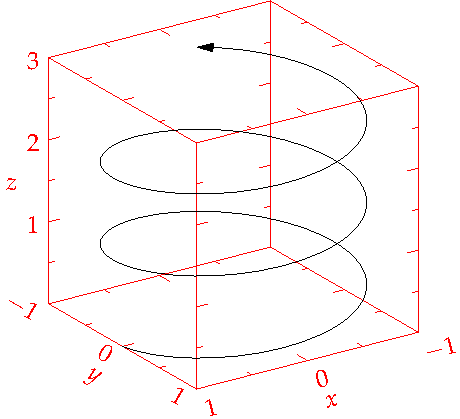
\includegraphics[width=\linewidth]{helix}
  \caption{This is a margin figure.  The helix is defined by 
    $x = \cos(2\pi z)$, $y = \sin(2\pi z)$, and $z = [0, 2.7]$.  The figure was
    drawn using Asymptote (\url{http://asymptote.sf.net/}).}
  \label{fig:marginfig}
\end{marginfigure}

\begin{docspec}
\textbackslash begin\{marginfigure\}\\
  \qquad\textbackslash includegraphics\{helix\}\\
  \qquad\textbackslash caption\{This is a margin figure.\}\\
  \qquad\textbackslash label\{fig:marginfig\}\\
\textbackslash end\{marginfigure\}\\
\end{docspec}

The \docenv{marginfigure} and \docenv{margintable} environments accept an optional parameter \docopt{offset} that adjusts the vertical position of the figure or table.  See the ``\nameref{sec:sidenotes}'' section above for examples.  The specifications are:
\begin{docspec}
  \textbackslash{begin\{marginfigure\}[\docopt{offset}]}\\
  \qquad\ldots\\
  \textbackslash{end\{marginfigure\}}\\
  \mbox{}\\
  \textbackslash{begin\{margintable\}[\docopt{offset}]}\\
  \qquad\ldots\\
  \textbackslash{end\{margintable\}}\\
\end{docspec}

Figure~\ref{fig:fullfig} is an example of the \docenv{figure*}
environment and figure~\ref{fig:textfig} is an example of the normal
\docenv{figure} environment.

\begin{figure*}[h]
  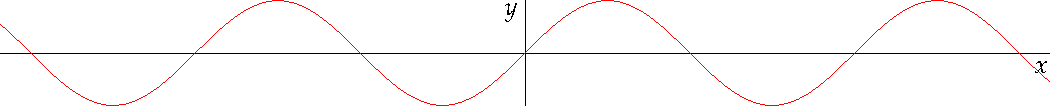
\includegraphics[width=\linewidth]{sine.pdf}%
  \caption{This graph shows $y = \sin x$ from about $x = [-10, 10]$.
  \emph{Notice that this figure takes up the full page width.}}%
  \label{fig:fullfig}%
\end{figure*}\FloatBarrier
\begin{figure}
  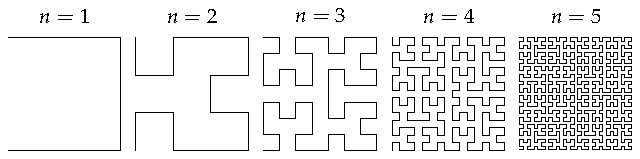
\includegraphics{hilbertcurves.pdf}
%  \checkparity This is an \pageparity\ page.%
  \caption[Hilbert curves of various degrees $n$.][6pt]{Hilbert curves of various degrees $n$. \emph{Notice that this figure only takes up the main textblock width.}}
  \label{fig:textfig}
  %\zsavepos{pos:textfig}
\end{figure}

As with sidenotes and marginnotes, a caption may sometimes require vertical
adjustment. The \doccmddef{caption} command now takes a second optional
argument that enables you to do this by providing a dimension \docopt{offset}.
You may specify the caption in any one of the following forms:
\begin{docspec}
  \doccmd{caption}\{\docarg{long caption}\}\\
  \doccmd{caption}[\docarg{short caption}]\{\docarg{long caption}\}\\
  \doccmd{caption}[][\docopt{offset}]\{\docarg{long caption}\}\\
  \doccmd{caption}[\docarg{short caption}][\docopt{offset}]%
                  \{\docarg{long caption}\}
\end{docspec}
A positive \docopt{offset} will push the caption down the page. The short
caption, if provided, is what appears in the list of figures/tables, otherwise
the ``long'' caption appears there. Note that although the arguments
\docopt{short caption} and \docopt{offset} are both optional, they must be
provided in order. Thus, to specify an \docopt{offset} without specifying a
\docopt{short caption}, you must include the first set of empty brackets
\Verb|[]|, which tell \doccmd{caption} to use the default ``long'' caption. As
an example, the caption to figure~\ref{fig:textfig} above was given in the form
\begin{docspec}
  \doccmd{caption}[Hilbert curves...][6pt]\{Hilbert curves...\}
\end{docspec}

Table~\ref{tab:normaltab} shows table created with the \docpkg{booktabs}
package.  Notice the lack of vertical rules---they serve only to clutter
the table's data.

\begin{table}[ht]
  \centering
  \fontfamily{ppl}\selectfont
  \begin{tabular}{ll}
    \toprule
    Margin & Length \\
    \midrule
    Paper width & \unit[8\nicefrac{1}{2}]{inches} \\
    Paper height & \unit[11]{inches} \\
    Textblock width & \unit[6\nicefrac{1}{2}]{inches} \\
    Textblock/sidenote gutter & \unit[\nicefrac{3}{8}]{inches} \\
    Sidenote width & \unit[2]{inches} \\
    \bottomrule
  \end{tabular}
  \caption{Here are the dimensions of the various margins used in the Tufte-handout class.}
  \label{tab:normaltab}
  %\zsavepos{pos:normaltab}
\end{table}

\newthought{Occasionally} \LaTeX{} will generate an error message:\label{err:too-many-floats}
\begin{docspec}
  Error: Too many unprocessed floats
\end{docspec}
\LaTeX{} tries to place floats in the best position on the page.  Until it's
finished composing the page, however, it won't know where those positions are.
If you have a lot of floats on a page (including sidenotes, margin notes,
figures, tables, etc.), \LaTeX{} may run out of ``slots'' to keep track of them
and will generate the above error.

\LaTeX{} initially allocates 18 slots for storing floats.  To work around this
limitation, the \TL document classes provide a \doccmddef{morefloats} command
that will reserve more slots.

The first time \doccmd{morefloats} is called, it allocates an additional 34
slots.  The second time \doccmd{morefloats} is called, it allocates another 26
slots.

The \doccmd{morefloats} command may only be used two times.  Calling it a
third time will generate an error message.  (This is because we can't safely
allocate many more floats or \LaTeX{} will run out of memory.)

If, after using the \doccmd{morefloats} command twice, you continue to get the
\texttt{Too many unprocessed floats} error, there are a couple things you can
do.

The \doccmddef{FloatBarrier} command will immediately process all the floats
before typesetting more material.  Since \doccmd{FloatBarrier} will start a new
paragraph, you should place this command at the beginning or end of a
paragraph.

The \doccmddef{clearpage} command will also process the floats before
continuing, but instead of starting a new paragraph, it will start a new page.

You can also try moving your floats around a bit: move a figure or table to the
next page or reduce the number of sidenotes.  (Each sidenote actually uses
\emph{two} slots.)

After the floats have placed, \LaTeX{} will mark those slots as unused so they
are available for the next page to be composed.

\section{Captions}
You may notice that the captions are sometimes misaligned.
Due to the way \LaTeX's float mechanism works, we can't know for sure where it
decided to put a float. Therefore, the \TL document classes provide commands to
override the caption position.

\paragraph{Vertical alignment} To override the vertical alignment, use the
\doccmd{setfloatalignment} command inside the float environment.  For
example:

\begin{fullwidth}
\begin{docspec}
  \textbackslash begin\{figure\}[btp]\\
  \qquad \textbackslash includegraphics\{sinewave\}\\
  \qquad \textbackslash caption\{This is an example of a sine wave.\}\\
  \qquad \textbackslash label\{fig:sinewave\}\\
  \qquad \hlred{\textbackslash setfloatalignment\{b\}\% forces caption to be bottom-aligned}\\
  \textbackslash end\{figure\}
\end{docspec}
\end{fullwidth}

\noindent The syntax of the \doccmddef{setfloatalignment} command is:

\begin{docspec}
  \doccmd{setfloatalignment}\{\docopt{pos}\}
\end{docspec}

\noindent where \docopt{pos} can be either \texttt{b} for bottom-aligned
captions, or \texttt{t} for top-aligned captions.

\paragraph{Horizontal alignment}\label{par:overriding-horizontal}
To override the horizontal alignment, use either the \doccmd{forceversofloat}
or the \doccmd{forcerectofloat} command inside of the float environment.  For
example:

\begin{fullwidth}
\begin{docspec}
  \textbackslash begin\{figure\}[btp]\\
  \qquad \textbackslash includegraphics\{sinewave\}\\
  \qquad \textbackslash caption\{This is an example of a sine wave.\}\\
  \qquad \textbackslash label\{fig:sinewave\}\\
  \qquad \hlred{\textbackslash forceversofloat\% forces caption to be set to the left of the float}\\
  \textbackslash end\{figure\}
\end{docspec}
\end{fullwidth}

The \doccmddef{forceversofloat} command causes the algorithm to assume the
float has been placed on a verso page---that is, a page on the left side of a
two-page spread.  Conversely, the \doccmddef{forcerectofloat} command causes
the algorithm to assume the float has been placed on a recto page---that is, a
page on the right side of a two-page spread.


\section{Full-width text blocks}

In addition to the new float types, there is a \docenvdef{fullwidth}
environment that stretches across the main text block and the sidenotes
area.

\begin{Verbatim}
\begin{fullwidth}
Lorem ipsum dolor sit amet...
\end{fullwidth}
\end{Verbatim}

\begin{fullwidth}
\small\itshape\lipsum[1]
\end{fullwidth}

\section{Typography}\label{sec:typography}

\subsection{Typefaces}\label{sec:typefaces}\index{typefaces}
If the Palatino, \textsf{Helvetica}, and \texttt{Bera Mono} typefaces are installed, this style
will use them automatically.  Otherwise, we'll fall back on the Computer Modern
typefaces.

\subsection{Letterspacing}\label{sec:letterspacing}
This document class includes two new commands and some improvements on
existing commands for letterspacing.

When setting strings of \allcaps{ALL CAPS} or \smallcaps{small caps}, the
letter\-spacing---that is, the spacing between the letters---should be
increased slightly.\cite{Bringhurst2005}  The \doccmddef{allcaps} command has proper letterspacing for
strings of \allcaps{FULL CAPITAL LETTERS}, and the \doccmddef{smallcaps} command
has letterspacing for \smallcaps{small capital letters}.  These commands
will also automatically convert the case of the text to upper- or
lowercase, respectively.

The \doccmddef{textsc} command has also been redefined to include
letterspacing.  The case of the \doccmd{textsc} argument is left as is,
however.  This allows one to use both uppercase and lowercase letters:
\textsc{The Initial Letters Of The Words In This Sentence Are Capitalized.}



\section{Document Class Options}\label{sec:options}

\index{class options|(}
The \doccls{tufte-book} class is based on the \LaTeX\ \doccls{book}
document class.  Therefore, you can pass any of the typical book
options.  There are a few options that are specific to the
\doccls{tufte-book} document class, however.

The \docclsoptdef{a4paper} option will set the paper size to \smallcaps{A4} instead of
the default \smallcaps{US} letter size.

The \docclsoptdef{sfsidenotes} option will set the sidenotes and title block in a 
\textsf{sans serif} typeface instead of the default roman.

The \docclsoptdef{twoside} option will modify the running heads so that the page
number is printed on the outside edge (as opposed to always printing the page
number on the right-side edge in \docclsoptdef{oneside} mode).  

The \docclsoptdef{symmetric} option typesets the sidenotes on the outside edge of
the page.  This is how books are traditionally printed, but is contrary to
Tufte's book design which sets the sidenotes on the right side of the page.
This option implicitly sets the \docclsopt{twoside} option.

The \docclsoptdef{justified} option sets all the text fully justified (flush left
and right).  The default is to set the text ragged right.  
The body text of Tufte's books are set ragged right.  This prevents
needless hyphenation and makes it easier to read the text in the slightly
narrower column.

The \docclsoptdef{bidi} option loads the \docpkg{bidi} package which is used with
\tXeLaTeX\ to typeset bi-directional text.  Since the \docpkg{bidi}
package needs to be loaded before the sidenotes and cite commands are defined,
it can't be loaded in the document preamble.

The \docclsoptdef{debug} option causes the \TL classes to output debug
information to the log file which is useful in troubleshooting bugs.  It will
also cause the graphics to be replaced by outlines.

The \docclsoptdef{nofonts} option prevents the \TL classes from
automatically loading the Palatino and Helvetica typefaces.  You should use
this option if you wish to load your own fonts.  If you're using \tXeLaTeX, this
option is implied (\ie, the Palatino and Helvetica fonts aren't loaded if you
use \tXeLaTeX).  

The \docclsoptdef{nols} option inhibits the letterspacing code.  The \TL\
classes try to load the appropriate letterspacing package (either pdf\TeX's
\docpkg{letterspace} package or the \docpkg{soul} package).  If you're using
\tXeLaTeX\ with \docpkg{fontenc}, however, you should configure your own
letterspacing.  

The \docclsoptdef{notitlepage} option causes \doccmd{maketitle} to generate a title
block instead of a title page.  The \doccls{book} class defaults to a title
page and the \doccls{handout} class defaults to the title block.  There is an
analogous \docclsoptdef{titlepage} option that forces \doccmd{maketitle} to
generate a full title page instead of the title block.

The \docclsoptdef{notoc} option suppresses \TL's custom table of contents
(\textsc{toc}) design.  The current \textsc{toc} design only shows unnumbered
chapter titles; it doesn't show sections or subsections.  The \docclsopt{notoc}
option will revert to \LaTeX's \textsc{toc} design.

The \docclsoptdef{nohyper} option prevents the \docpkg{hyperref} package from
being loaded.  The default is to load the \docpkg{hyperref} package and use the
\doccmd{title} and \doccmd{author} contents as metadata for the generated
\textsc{pdf}.

\index{class options|)}


\chapter{Receiver Operating Characteristic ROC Curves}
\label{ch:roc-curves}\index{roc-curves}

\section{Introduction}
A Receiver Operating Characteristic (ROC) curve is a graphical plot which presents the performance of a binary classifier when the discrimination cut-off, or threshold\index{roc-curves!threshold}, is varied. The ROC curves and associated analysis, such as area under the curve, comparing multiple ROC curves and finding an optimal threshold, have proved very useful analysis tools in many fields of research such as medical diagnosis and disease management. They have been found to be a more appropriate technique for evaluating diagnostic and predictive accuracy.

Essentially for creating and plotting the ROC curve one needs to compute the true positive rate (TPR)\index{roc-curves!true positive rate} and the false positive rate (FPR)\index{roc-curves!false positive rate} at various threshold settings and plot them in a dimensional space. In machine learning the TPR is referred to as the sensitivity\index{roc-curves!sensitivity} or recall which measures the proportion of actual positives that are correctly classified. The true negative rate (TNR)\index{roc-curves!true negative rate}, or specificity\index{roc-curves!specificity}, measures the proportion of actual negatives that are correctly identified as such. These measures can be easily summarised in Table 1 below.

\begin{table}[]
	\begin{tabular}{|l|cc|ll|}
		\hline
		\multicolumn{1}{|c|}{\textbf{Predicted Class}} & \multicolumn{2}{c|}{\textbf{True Class}}                                                                              &              &                       \\ \hline
		Yes / 1 / Positive                             & True Positives                                            & \begin{tabular}[c]{@{}c@{}}False\\ Positives\end{tabular} & TPR = TP / P & Sensitivity = TPR     \\
		No / 0 / Negative                              & \begin{tabular}[c]{@{}c@{}}False\\ Negatives\end{tabular} & True Negatives                                            & FPR = FP / N & Specificity = 1 - FPR \\ \hline
		& \textbf{P}                                                & \textbf{N}                                                &              &                       \\ \hline
	\end{tabular}
	\caption{\label{tab:sens-spec}Sensitivity and specificity}
\end{table}

ROC curves are widely used in medical applications. Consider a diagnostic test that seeks to determine whether a person has a certain disease. This is a two-class prediction problem in which the outcome is labelled either positive or negative. In this case there are four possible outcomes from the discrete classifier: true positive or true negative if the outcome matches the actual class, false positive if the person is incorrectly classified as sick, and false negative if the person is incorrectly classified as healthy. If the test is extended to a larger sample then given a classifier and a set of instances, a 2x2 contingency table\index{roc-curves!contingency table}, or confusion matrix, can be constructed representing the dispositions of the set of instances. Extending the test further to five classifiers, A to E, an ROC curve can be plotted, figure 1 (adopted from \citep{fawcett2006introroc}), with TPR on the y-axis and FPR (or 1 – specificity) on x-axis, which defines our ROC space depicting the relative trade-offs between true positives (benefits) and false positives (costs). 

The diagonal line from (0,0) to (1,1) characterises a test that cannot distinguish between diseased and non-diseased states, that is, a random guess. This line often serves as a benchmark for judging how well (or bad) a test performs.

\begin{figure}
	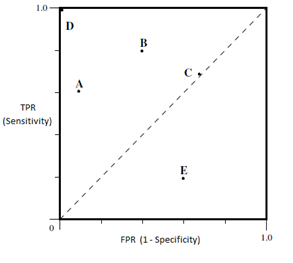
\includegraphics{roc_curves/Figure1.png}
	\caption{Basic ROC plot with five classifiers.}
	\label{fig:classifiers-roc}
\end{figure}

\section{Evaluating Classifiers} \index{roc-curves!evaluating classifiers}
The best possible prediction method would yield a point in the upper left corner of the ROC space representing 100\% sensitivity and 100\% specificity, i.e. a perfect classifier. On the other hand, a random guess would outcome a point along or close to the diagonal line. Classifiers A and B yield good classification results whilst points below the line represent bad results (worse than random). The ROC plot allows us to compare classifiers and choose the one that is closest to (0,1) and furthest from TPR equals FPR (the diagonal line).

Consider now that the blood protein levels in diseased people and healthy people are normally distributed. A medical test might measure the level of a certain protein in a blood sample and classify any number above a certain threshold as indicating disease. Thus given a threshold parameter $p$, the instance is labelled positive if the continuous random variable $X$ is greater than $p$ and negative otherwise. As shown in figure 2 (left), choosing a high threshold produces a low likelihood of a false positive (while increasing the specificity) and a high likelihood of a false negative result (while decreasing sensitivity). Choosing a low threshold results in the opposite effect. Thus a different threshold would result in a different sensitivity and specificity pair. By repeating the experiment with adjusted thresholds different values for FPR and TPR are obtained leading to different positioning in the ROC space. The classifier that is able to increase the rate of detection while keeping the false alarm rate low is considered a good classifier. Figure 2 (right) shows the ROC curves with different thresholds. As the ROC curve gets closer to the top left hand of the graph the more optimal the threshold and the better the ability to discriminate between the classes.

\begin{figure}
	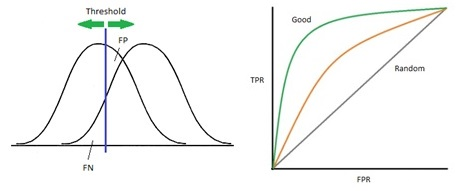
\includegraphics{roc_curves/Figure2.png}
	\caption{Left: Distributions of results for a hypothetical continuous diagnostic test. Right: ROC curves with different thresholds.}
	\label{fig:roc-curves}
\end{figure}

\section{Area Under Curve} \index{roc-curves!area Under curve}
The most common condition for choosing the optimal parameterisation is to maximise the area under the curve, AUC for short. The AUC, defined as $\int_{0}^{1} ROC(t) dt$ is a widely used measure of performance of supervised classification rules. It is a measure of the usefulness, or rather the discriminatory ability, of a test in general where the greater the area the more discriminative\index{roc-curves!discriminative} the test is in a given situation. A model or test with perfect discriminatory ability will have an AUC of, or very close to, 1.0, while a model unable to distinguish between individuals with or without the chosen outcome will have an AUC value of 0.5.  No realistic classifier should have an AUC less than 0.5. 

\begin{marginfigure}
	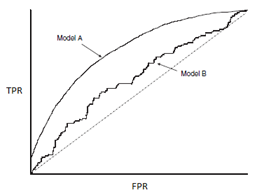
\includegraphics{roc_curves/Figure3.png}
	\caption{A comparison of two AUC curves.}
	\label{fig:two-curves}
\end{marginfigure}

However, the true value of AUC comes when comparing two or more models or tests by reducing the ROC to a single scalar value representing the expected performance of the models. Figure 3 (adopted from \citep{linden2006diagpreddismgmt}) provides a comparison between two predictive models. Model A is both statistically and visually better at identifying individuals with and without the outcome than Model B since the AUC is bigger. Therefore, if a choice was to be made between selecting one of the models, Model A would be the choice.

AUC is a desirable measure because (1) it is scale-invariant\index{roc-curves!scale-invariant}: it measures how well predictions are ranked rather than their absolute values; (2) AUC is classification-threshold-invariant\index{roc-curves!classification-threshold-invariant}: it measures the quality of the model’s predictions irrespective of the classification threshold chosen.

\section{Multi-class ROC} \index{roc-curves!multi-class roc}
ROC curves are typically used in binary classification problems but what about multi-class problems? In order to extend ROC analysis to multi-class or multi-label classification, it is necessary to binarise the output. A multi-class problem introduces the issue of combining pairwise discriminability values. One approach introduced by Provost and Domingos \citep{provost2003treeind} was to generate each class reference ROC curve, in turn measure the AUC, then assuming the AUCs are weighted by the reference class’s prevalence in the data. More precisely, $AUC_{total} = \sum AUC(c_{i}).p(c_{i})$ where $c_{i}\in C$ the set of all thresholds, and $p$ is the probability of class membership.
The disadvantage with this method is that the class reference ROC is sensitive to class distributions and error costs, so is the formulation of $AUC_{total}$.

To overcome this problem Hand and Till \citep{hand2001aucmulticlass} suggested a derivation that is based on the fact that the classifier will rank a randomly chosen positive instance higher than a randomly chosen negative instance. From this probabilistic form, they derived a formulation that measures the unweighted pairwise discriminability of classes. While this formulation is well justified and is insensitive to changes in the class distribution, they found no easy way to visualise the surface whose area is being calculated.

Thanks to its close relationship with yet another widespread Wilcoxon statistic \citep{hanley1982useauc}, AUC methods for AUC-based analyses are well developed and widely used. However one of the major practical drawbacks of the AUC as an index of diagnostic performance\index{roc-curves!diagnostic performance} is that it summarises the entire ROC curve including the regions that frequently are not relevant to practical applications, such as regions with low level of specificity, according to Ma et al. 2013 \citep{ma2013paucdiagperf}. To alleviate this deficiency while benefiting from some of the advantageous properties of the area under the ROC curve, one can use a partial area under the curve (pAUC for short), which summarizes a portion of the curve over the prespecified range of interest. A number of approaches have been developed for pAUC-based analysis \citep{dodd2003pauc,he2010nonparagenomic,mcclish1989paucanal,zhang2002nonparpaucapp}. However, Ma et al. argue that the same features that increase the practical relevance of the pAUC introduce some difficulty to resolve issues related to arbitrariness of specifying the range of interest. 

\begin{marginfigure}
	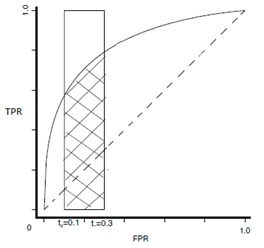
\includegraphics{roc_curves/Figure4.png}
	\caption{Illustration of an ROC curve and its partial AUC with $t_{0}$ = 0.1 and $t_{1}$ = 0.3.}
	\label{fig:partial-auc}
\end{marginfigure}

\section{Partial AUC} \index{roc-curves!partial area under curve}
Dodd and Pepe \citep{dodd2003pauc} claim that in population screening, in order to avoid high monetary costs the region of the curve corresponding to low false-positive rates is of primary interest. In diagnostic testing it is critical to maintain a high TPR in order not to miss detecting diseased subjects. They go on to consider a summary index for the ROC curve restricted to a clinically relevant range of false-positive rates.

Essentially the partial AUC is simply the area under the ROC curve between $t_{0}$ and $t_{1}$ (Figure 4) where the interval ($t_{0},t_{1}$) denotes the false-positive rates of interest. The partial AUC is thus the integral between $t_{0}$ and $t_{1}$ of the ROC curve function as shown in equation 1.

\begin{equation}\label{eq:partial-auc}
AUC(t_{0},t_{1}) = \int_{t_{0}}^{t_{1}} ROC(t)  dt
\end{equation}

Selecting the interval is an important practical issue but it is beyond the scope of this essay to delve further.

\section{Applications of ROC}
ROC curves have been used by numerous authors to evaluate models and scoring systems developed for pest risk assessment \citep{copp2009screening,heidy2010minfneginvspec}. They conclude that, in comparison with other models, the strength of the ROC analysis is that it thoroughly investigates test accuracy\index{roc-curves!test accuracy} across a range of scores, and that it allows for visual examination of scores on one curve or a comparison of two or more curves using a similar metric. This allows analysts to easily determine which decision threshold is most preferred, based on the desired trade-off between sensitivity and specificity, or to establish which model has the best accuracy based on the largest AUC \citep{linden2006diagpreddismgmt}. In a later paper Makowski and Mittinty \citep{makowski2010scorsysinvpests} present a procedure based on Monte Carlo simulations and ROC analysis to assess and compare scoring systems for invasive species. In their methodology the process model is a stochastic model simulating the invasion process, the candidate models are the scoring systems and the metric is the area under the ROC curve.

An interesting recent paper by Fung et al. \citep{fung2018cnnbcancerclass} evidences how ROC curves statistics are used to evaluate Convolutional Neural Network for breast cancer classification. It compares the ROC curves generated from the classifier with other reviewed studies. The analysis of AUC helped in evaluating the superiority of the neural network to the compared methods based on experimental results conducted on real patient subjects.

Another field where ROC proves to be contributory is psychology. Correct identification of criminals by eyewitness can help to remove a dangerous criminal from society but a false identification can lead to the erroneous conviction of an innocent suspect. A 2014 paper by Gronlund et al. \citep{gronlund2014eyewitness} describes how constructing ROC curves researchers can trace out discriminability across levels of response bias for each lineup procedure. They illustrate the shortcomings of ratio-based measures and demonstrate why ROC analysis is required for evaluating the performance of a lineup procedure. In a more recent paper Luby \citep{luby2017lineup} goes a step further and examines the application of ROC methodology to lineup data and shows that by using a log-linear analysis in conjunction with an ROC approach to eyewitness identification it is possible not only to visualise the trade-off between true positives and false positives, but also to identify which variables are interacting with one another to explain the trade-off.

\section{Final Note on History}
A final note on the history of ROC. The first use of ROC curves is traced back to World War II where in conjunction with signal detection theory, it developed for the analysis of radar images. Radar operators had to decide whether a blip on the radar screen represented and enemy target, a friendly ship or just noise. Signal detection theory measures the ability of radar receiver operators to make these important distinctions. Their ability to do so was called the Receiver Operating Characteristics. The introduction of ROC analysis into the biomedical field came in the 1970s via the radiological sciences where it has been used extensively to test the ability of an observer to discriminate between healthy and diseased subjects using a given diagnostic test, as well as to compare the efficacy among the various tests available. Since then ROC analysis has been extended for use in visualising and analysing the behaviour of a broad range of diagnostic systems across many fields of science. 

 %TODO


%%
% The back matter contains appendices, bibliographies, indices, glossaries, etc.

\backmatter

%% \bibliography{terms/myterm_jpe} 
\bibliography{terms/crossvalidation_lmd}
\bibliography{terms/roccurves_pb}
\bibliographystyle{plainnat}

\printindex

\end{document}

